\documentclass[11pt]{article}
\usepackage[T1]{fontenc}
\usepackage[utf8]{inputenc}
\usepackage[letterpaper]{geometry}

\usepackage{graphicx}
\usepackage{mathpazo}

\usepackage{amsmath}
\usepackage{amsfonts}
\usepackage{bm}
\usepackage{siunitx}
\usepackage{cancel}
\usepackage{float}
\usepackage{empheq}
\usepackage[most]{tcolorbox}

% Sexy yellow highlighted boxed equations!
\newtcbox{\mymath}[1][]{%
	nobeforeafter, math upper, tcbox raise base,
	enhanced, colframe=black!30!black,
	colback=yellow!30, boxrule=1pt,
	#1}

% Hyperlinks with decent looking default colors.
\usepackage{hyperref}
\usepackage{xcolor}
\hypersetup{
	colorlinks,
	linkcolor={red!50!black},
	citecolor={blue!50!black},
	urlcolor={blue!80!black}
}

% For those sexy spaced low small caps from classic-thesis!
\usepackage{microtype}
\usepackage{textcase}
\DeclareRobustCommand{\spacedlowsmallcaps}[1]{%
	\textls[80]{\scshape\MakeTextLowercase{#1}}%
}

% Replaced mathpazo \sum symbol with computer modern's.
\DeclareSymbolFont{cmlargesymbols}{OMX}{cmex}{m}{n}
\let\sumop\relax
\DeclareMathSymbol{\sumop}{\mathop}{cmlargesymbols}{"50}

% Force indent command.
\newcommand{\forceindent}{\leavevmode{\parindent=1em\indent}}

% Math shortcuts.
\newcommand\p[2]{\frac{\partial #1}{\partial #2}}

% fancyhdr header and footer.
\usepackage{fancyhdr}
\pagestyle{fancy} 
\fancyhead{}
\rhead{Ali Ramadhan}
\chead{}
\lhead{12.818: Project 8}
\cfoot{}
\rfoot{\thepage}

\title{\spacedlowsmallcaps{\small 12.818: Introduction to Atmospheric Data and Large-scale Dynamics}\\ \spacedlowsmallcaps{\Large Project eight: Estimation of vertical velocity}}
\author{\spacedlowsmallcaps{Ali Ramadhan}}
\date{}

\begin{document}
\maketitle

In this project, we will make estimates for the vertical velocity of air parcels in the atmosphere using two different methods, by inference from the vorticity equation and by the use of isentropic analysis.

\section{Estimation of vertical velocity from the vorticity equation}
As we saw in class, the vorticity equation
\begin{equation} \label{eq:voreq}
  f \p{\omega}{p} = \p{\zeta_g}{t} + \bm{u}_g \cdot \nabla (\zeta_g + f) + g \p{}{p} (\hat{\bm{z}} \cdot \nabla \times \bm{\tau})
\end{equation}
relates the change in vorticity to the difference in vertical velocity at the top and bottom of the column, and so if the vertical velocity at one end of the column is known, the vertical velocity at the other end can be inferred from the vorticity equation. Here, $\zeta_g + f$ is the absolute vorticity, $f$ is the planetary vorticity, $\zeta_g$ is the geostrophic relative vorticity evaluated on an isobaric surface, $\omega$ is the vertical velocity in pressure coordinates, $\bm{\tau}$ is the surface stress vector, $g$ is the acceleration due to gravity, and $\bm{u}_g$ is the geostrophic wind velocity field.

The $\p{\zeta_g}{t}$ term is the rate of change of relative vorticity (figure \ref{fig:dvordt_700hPa_MI}), while $\bm{u}_g \cdot \nabla (\zeta_g + f)$ represents the horizontal advection of absolute vorticity (figure \ref{fig:hor_adv_vor_MI_850hPa}) and $g \p{}{p} (\hat{\bm{z}} \cdot \nabla \times \bm{\tau})$ the destruction of vorticity by surface stress, which becomes significant only near the Earth's surface and so we won't consider it here. For this section, we will be looking at the Great Lakes region.

\begin{figure}[h!]
	\centering
	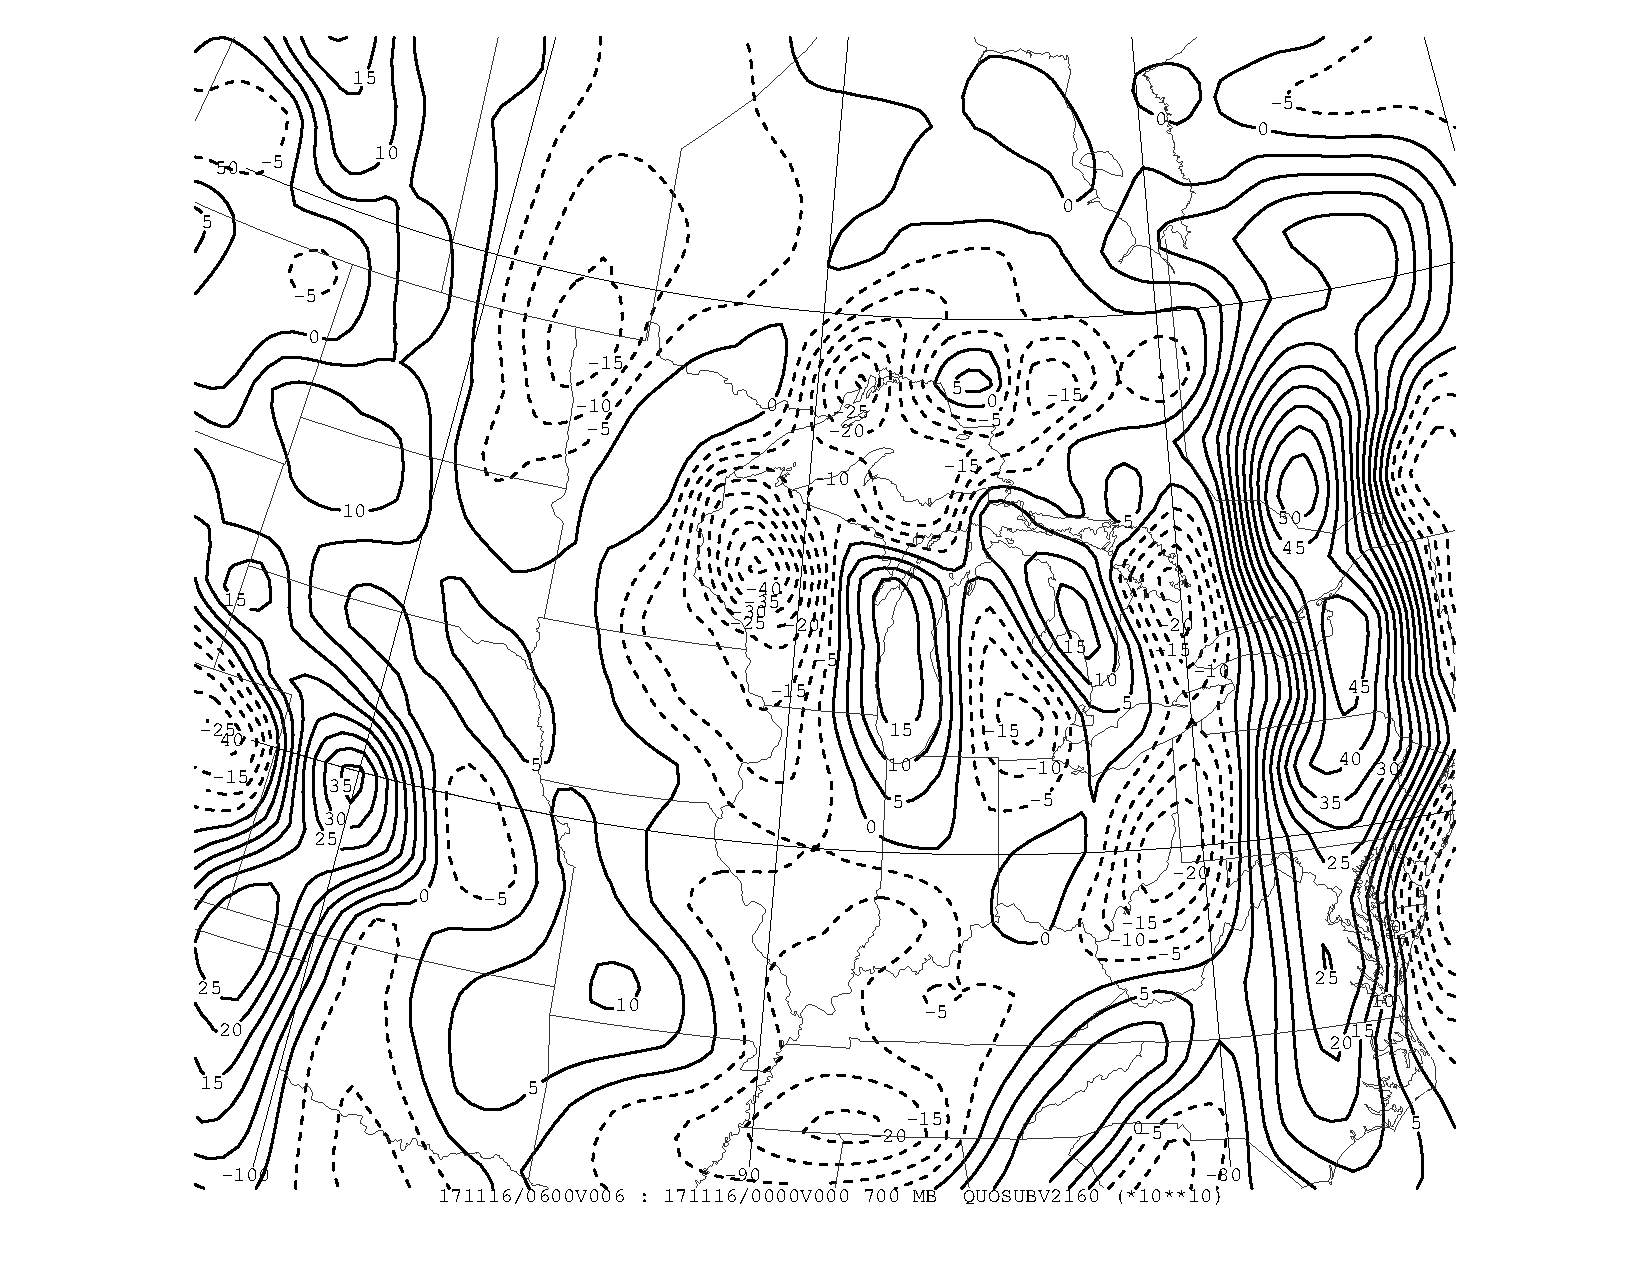
\includegraphics[width=\textwidth,trim={2.5cm 1cm 2.5cm 0},clip]{dvordt_700hPa_MI}
	\caption{Contour plot of the rate of change of relative vorticity ($\times \SI{e10}{\per\s\squared}$) at \SI{700}{\hecto\Pa} over the Great Lakes region between November 16, 2017 0Z and 6Z.}
	\label{fig:dvordt_700hPa_MI}
\end{figure}

\begin{figure}[h!]
  \centering
  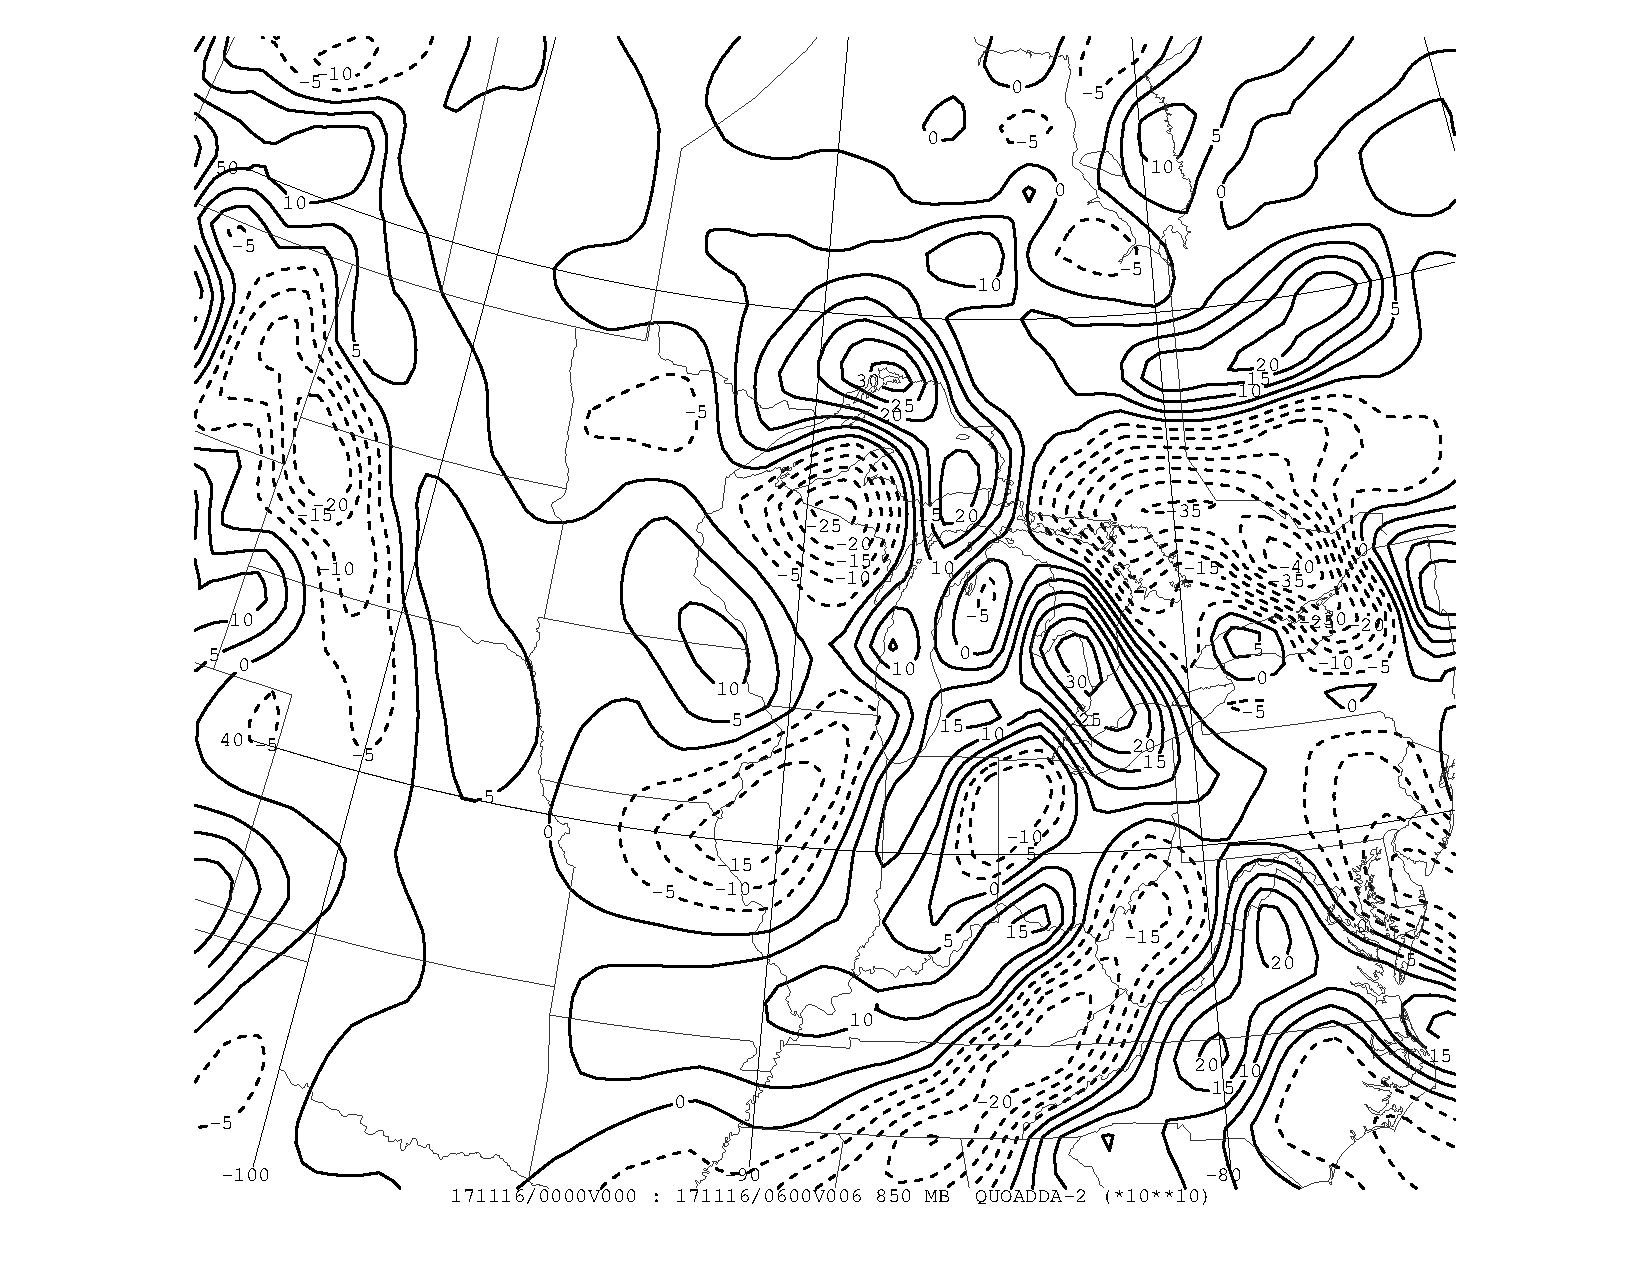
\includegraphics[width=\textwidth,trim={2.5cm 1cm 2.5cm 0},clip]{hor_adv_vor_MI_850hPa}
  \caption{Contour plot of the Horizontal advection of absolute vorticity ($\times \SI{e10}{\per\s\squared}$) at \SI{850}{\hecto\Pa} over the Great Lakes region between November 16, 2017 0Z and 6Z.}
  \label{fig:hor_adv_vor_MI_850hPa}
\end{figure}

\begin{figure}[h!]
  \centering
  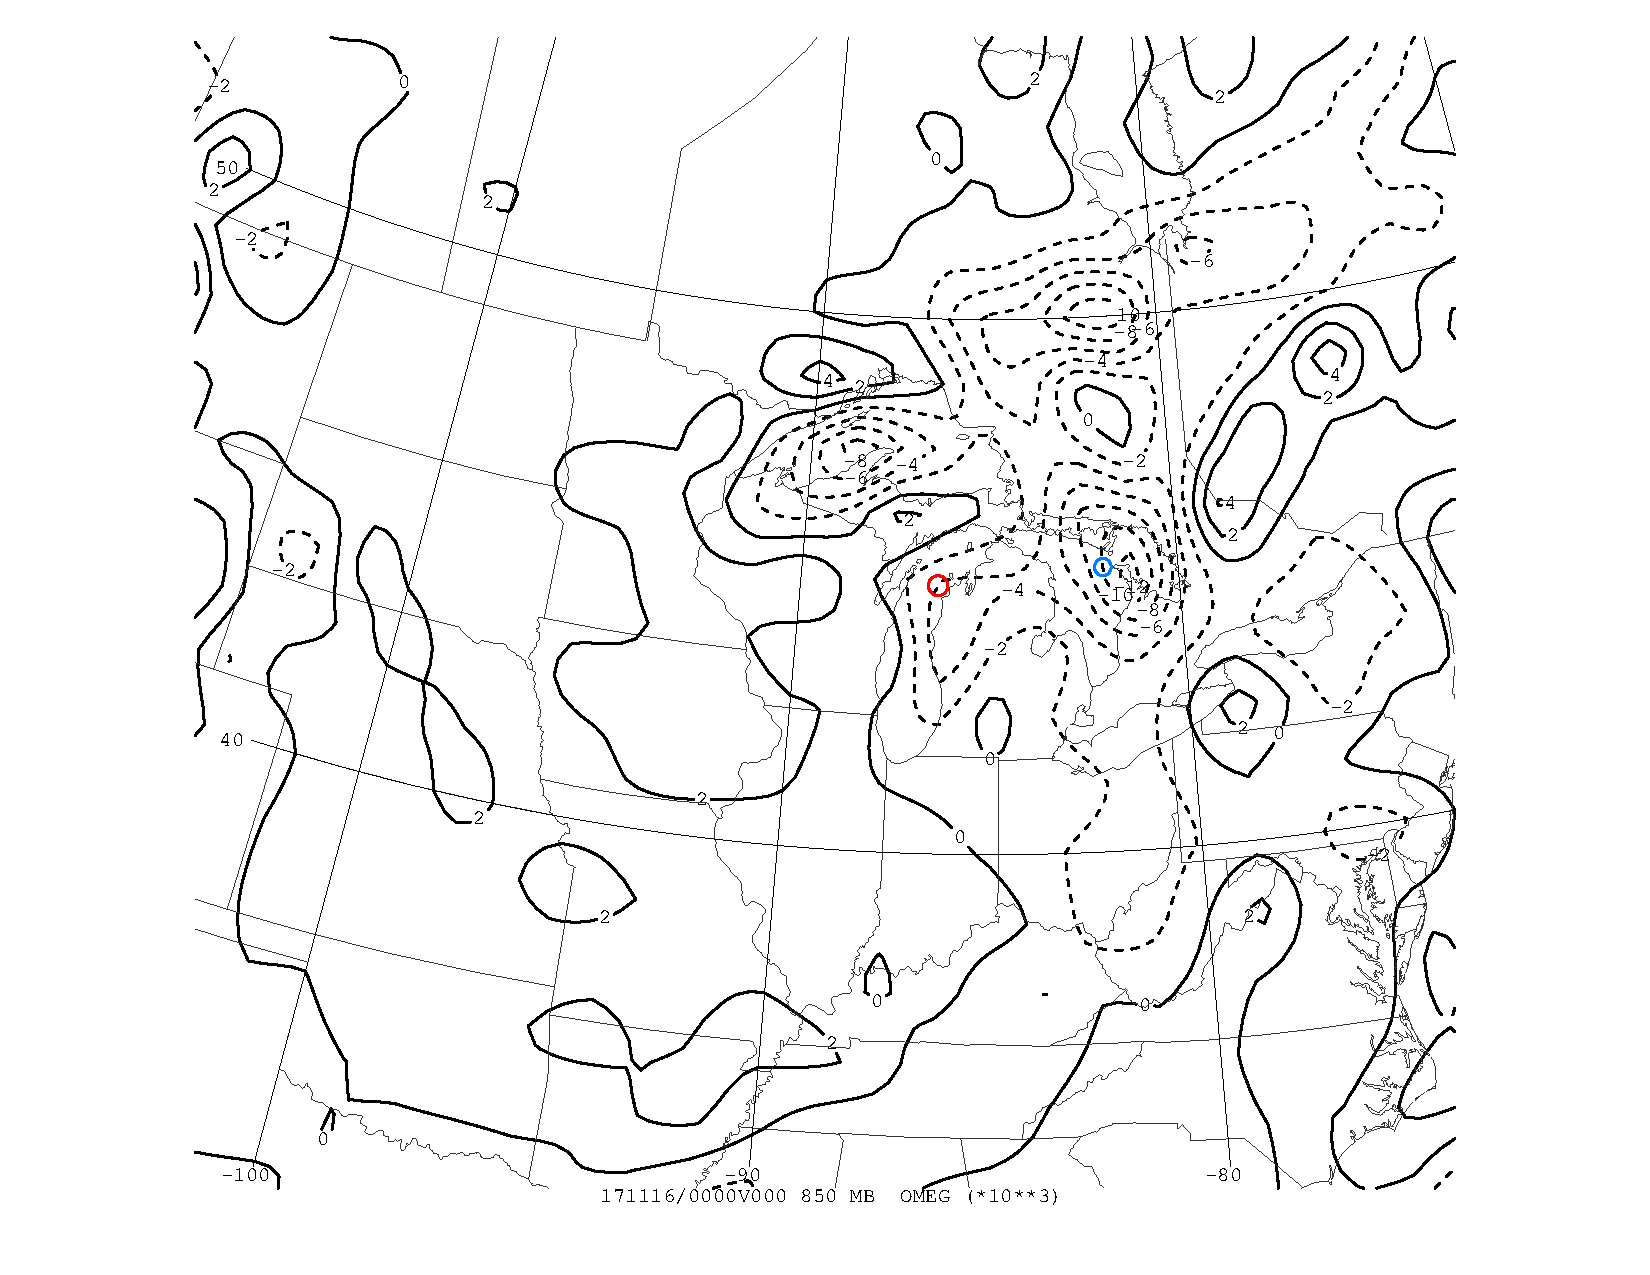
\includegraphics[width=\textwidth,trim={2.5cm 1cm 2.5cm 0},clip]{omega_MI_850hPa}
  \caption{Contour plot of the vertical velocity in pressure coordinates $\omega$ ($\times \SI{e3}{\hecto\Pa\per\s}$) at \SI{850}{\hecto\Pa} over the Great Lakes region between November 16, 2017 0Z and 6Z.}
  \label{fig:omega_MI_850hPa}
\end{figure}

Discretizing the $\partial \omega / \partial p$ derivative in \eqref{eq:voreq} using a first-order finite difference we get
\begin{equation*}
f \frac{\omega(\SI{850}{\hecto\Pa}) - \omega(\SI{700}{\hecto\Pa})}{\Delta p} = \p{\zeta_g}{t} + \bm{u}_g \cdot \nabla (\zeta_g + f) + \underbrace{g \p{}{p} (\hat{\bm{z}} \cdot \nabla \times \bm{\tau})}_\text{$=0$ near the Earth's surface}
\end{equation*}
where $\Delta p = \SI{850}{\hecto\Pa} - \SI{700}{\hecto\Pa} = \SI{150}{\hecto\Pa}$ and we are ignoring effects due to surface stresses and wind stress curl. Thus we can estimate the vertical velocity at \SI{700}{\hecto\Pa} from the vertical velocity at \SI{850}{\hecto\Pa} using
\begin{equation} \label{eq:voreq_fdiff}
\omega(\SI{700}{\hecto\Pa}) = \omega(\SI{850}{\hecto\Pa}) - \frac{\Delta p}{f} \left[ \p{\zeta_g}{t} + \bm{u}_g \cdot \nabla (\zeta_g + f) \right]
\end{equation}

We will use \eqref{eq:voreq_fdiff} and figures \ref{fig:dvordt_700hPa_MI}--\ref{fig:omega_MI_850hPa} to estimate the vertical velocity at two different locations, over Lake Michigan just off the west coast of Michigan (red circle in figure \ref{fig:omega_MI_850hPa}) and over Lake Huron off the east coast of Michigan close to the Georgian Bay (blue circle in figure \ref{fig:omega_MI_700hPa}). Over Lake Michigan we can estimate $\p{\zeta_g}{t} \approx \SI{15e-10}{\per\s\squared}$, $\bm{u}_g \cdot \nabla (\zeta_g + f) \approx \SI{7.5e-10}{\per\s\squared}$, and $\omega(\SI{850}{\hecto\Pa}) \approx \SI{-4e3}{\Pa\per\s}$, and so we estimate that $\omega(\SI{700}{\hecto\Pa}) \approx \SI{-4.4e3}{\hecto\Pa\per\s} = \SI{-4.4}{\Pa\per\s}$, which is pretty accurate as the point is inside the $-4$ contour at $\omega(\SI{700}{\hecto\Pa})$ (figure \ref{fig:omega_MI_700hPa}).

In between Lake Huron and the Georgian Bay we estimate $\p{\zeta_g}{t} \approx \SI{5e-10}{\per\s\squared}$, $\bm{u}_g \cdot \nabla (\zeta_g + f) \approx \SI{5e-10}{\per\s\squared}$, and $\omega(\SI{850}{\hecto\Pa}) \approx \SI{-10e3}{\Pa\per\s}$, and so we estimate that $\omega(\SI{700}{\hecto\Pa}) \approx \SI{-10.2e3}{\hecto\Pa\per\s} = \SI{-10.2}{\Pa\per\s}$, which is not very far off the obsrved value of $\sim \SI{-7}{\Pa\per\s}$ (see figure \ref{fig:omega_MI_700hPa}).

\begin{figure}[h!]
  \centering
  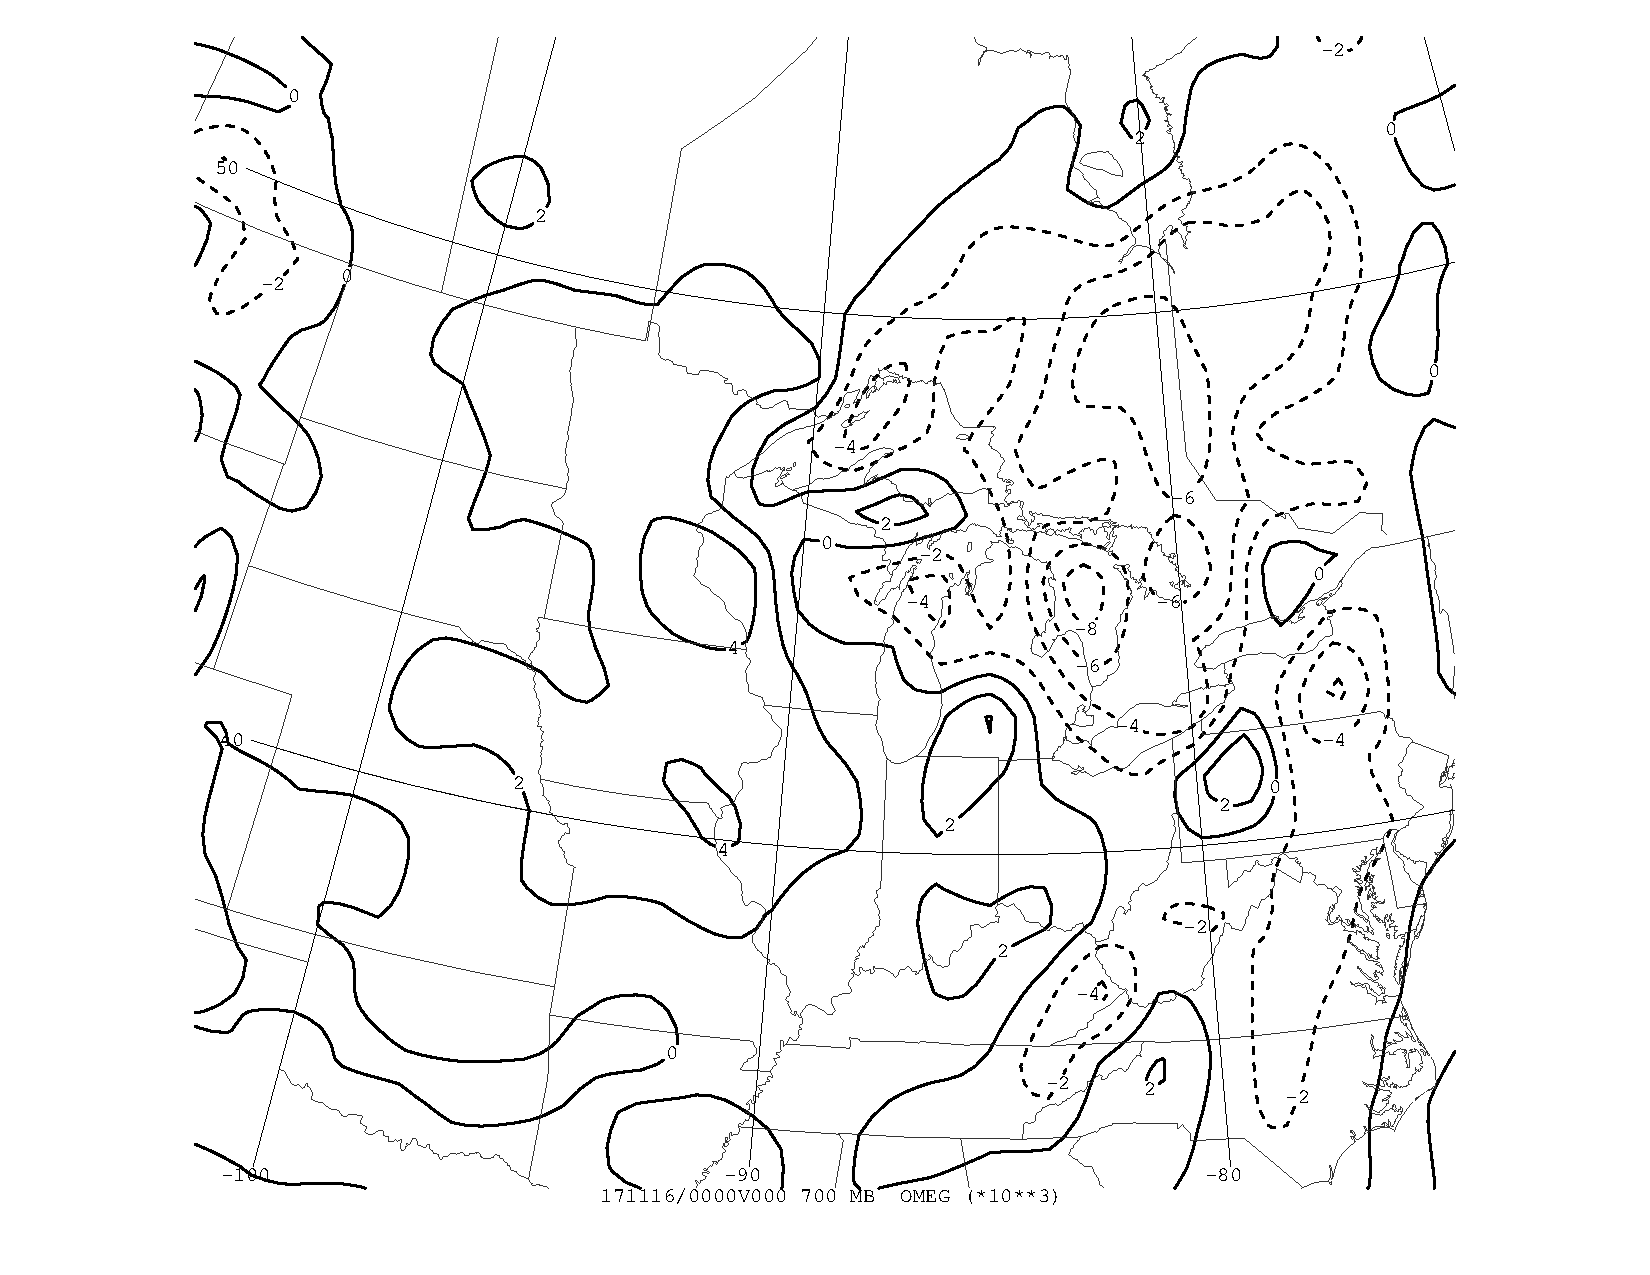
\includegraphics[width=\textwidth,trim={2.5cm 1cm 2.5cm 0},clip]{omega_MI_700hPa}
  \caption{Contour plot of the vertical velocity in pressure coordinates $\omega$ ($\times \SI{e3}{\hecto\Pa\per\s}$) at \SI{700}{\hecto\Pa} over the Great Lakes region between November 16, 2017 0Z and 6Z.}
  \label{fig:omega_MI_700hPa}
\end{figure}

I suppose a more accurate way of verifying our estimates would be to actually compute the $\omega(\SI{700}{\hecto\Pa})$ using \eqref{eq:voreq_fdiff} in GEMPACK and calculate the residual field between it and the observed field. An obvious advantage of producing a residual field is that we may investigate the question of where does this approximation work well and where does it fail.

\section{Estimation of vertical velocity using isentropic analysis}
Another method of estimating vertical velocities is by inference from isentropic analysis. The premise of this method relies on the fact that away from clouds, potential temperature is approximately convserved for air parcels and so their trajectories lie on an isentropic surface, i.e. a surface of constant entropy. We can obtain an estimate of the vertical velocity from the change in pressure level of the surface along such a trajectory as $\omega = dp/dt$.

The reason we chose to look at the Great Lakes region in the previous section was due to the presence of a low-pressure system over the Great Lakes region on November 16, 2017 0Z (clearly seen in figures \ref{fig:thta_pres_field_MI_0Z} and \ref{fig:thta_pres_field_MI_6Z}). The zonal cross-sections at 0Z and 6Z (figures \ref{fig:thta_171116_0Z_EW} and \ref{fig:thta_171116_6Z_EW}) and the meridional cross-sections at 0Z and 6Z (figure \ref{fig:thta_171116_0Z_NS_lon80W} and \ref{fig:thta_171116_6Z_NS}) all suggest that the \SI{300}{\K} potential temperature surface would be a suitable one to track air parcel trajectories on as the pressure changes significantly on it, providing us with a clear signal for which we can estimate vertical velocities.

\begin{figure}[h!]
  \centering
  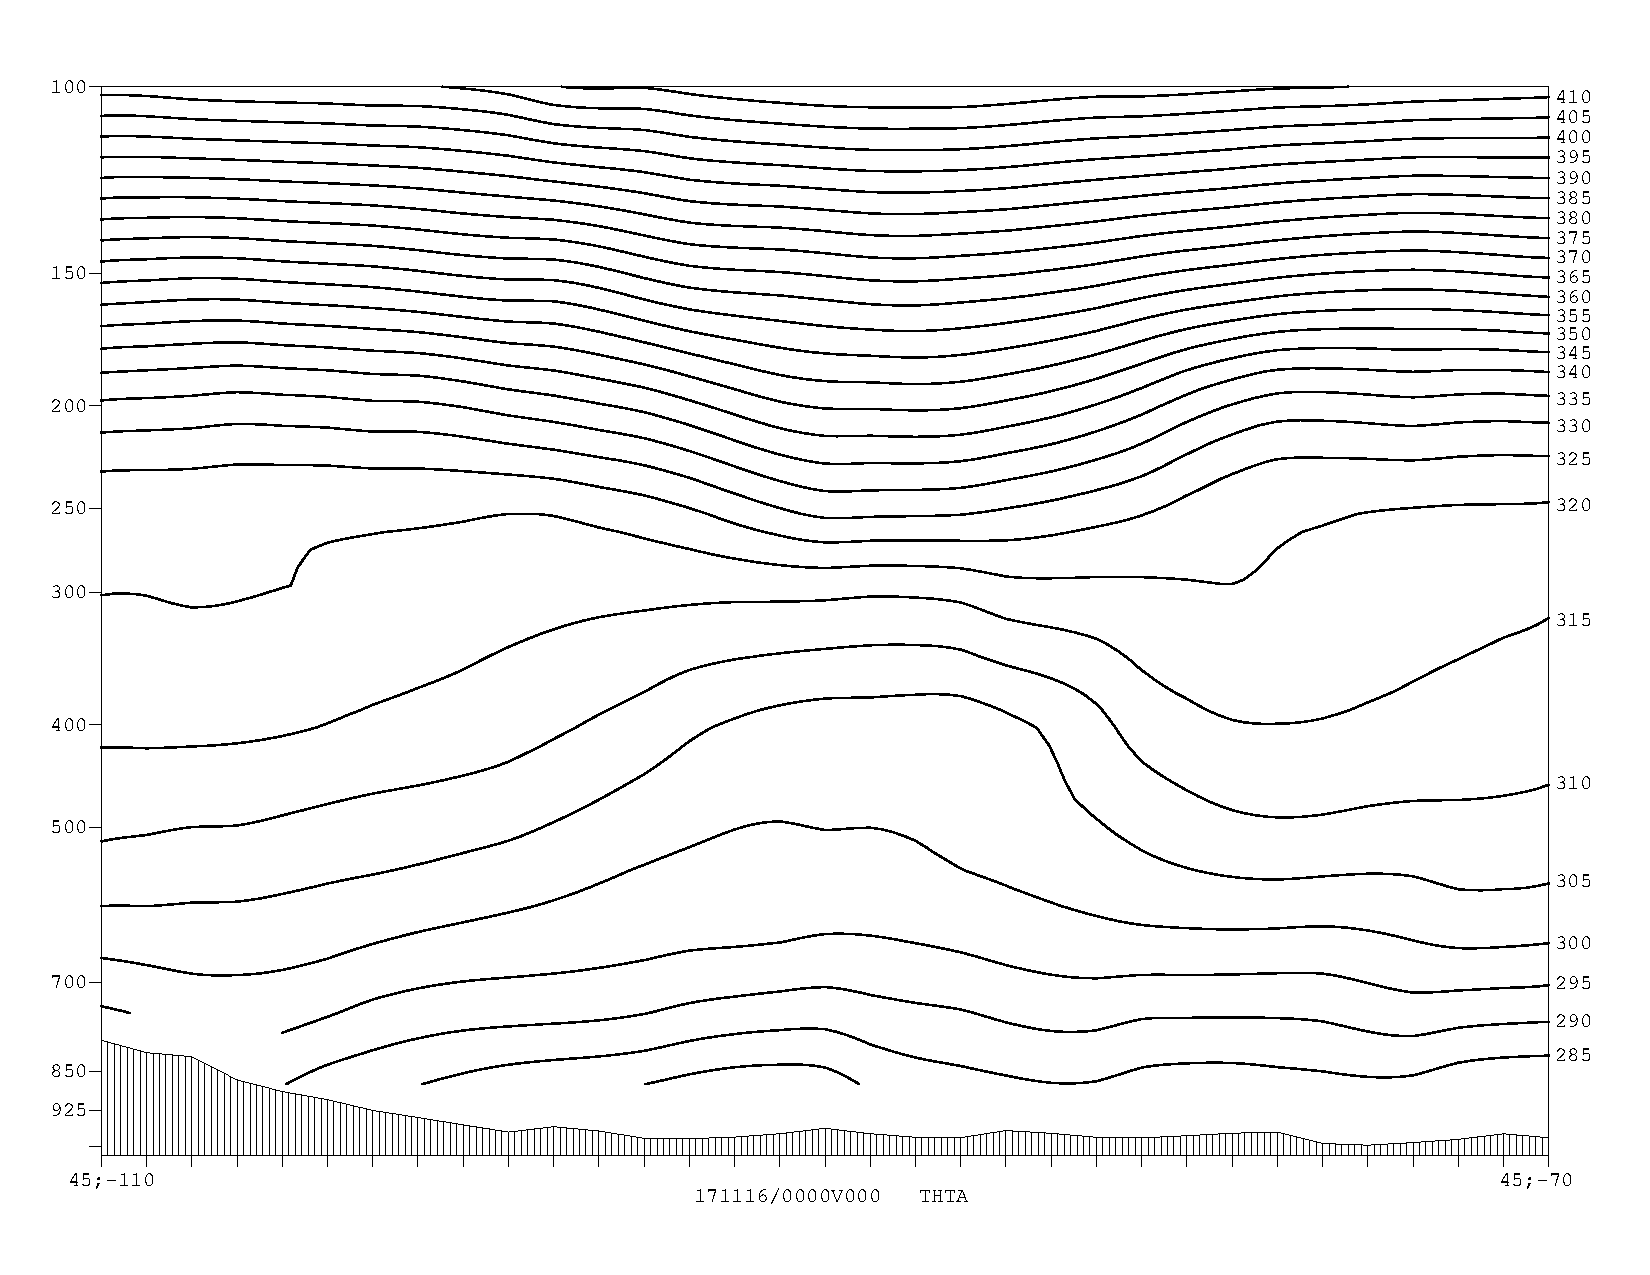
\includegraphics[width=\textwidth]{thta_171116_0Z_EW}
  \caption{Zonal cross-section of the potential temperature at \SI{45}{\degree N} and from \SI{110}{\degree W} to \SI{70}{\degree W} on November 16, 2017 0Z.}
  \label{fig:thta_171116_0Z_EW}
\end{figure}

\begin{figure}[h!]
  \centering
  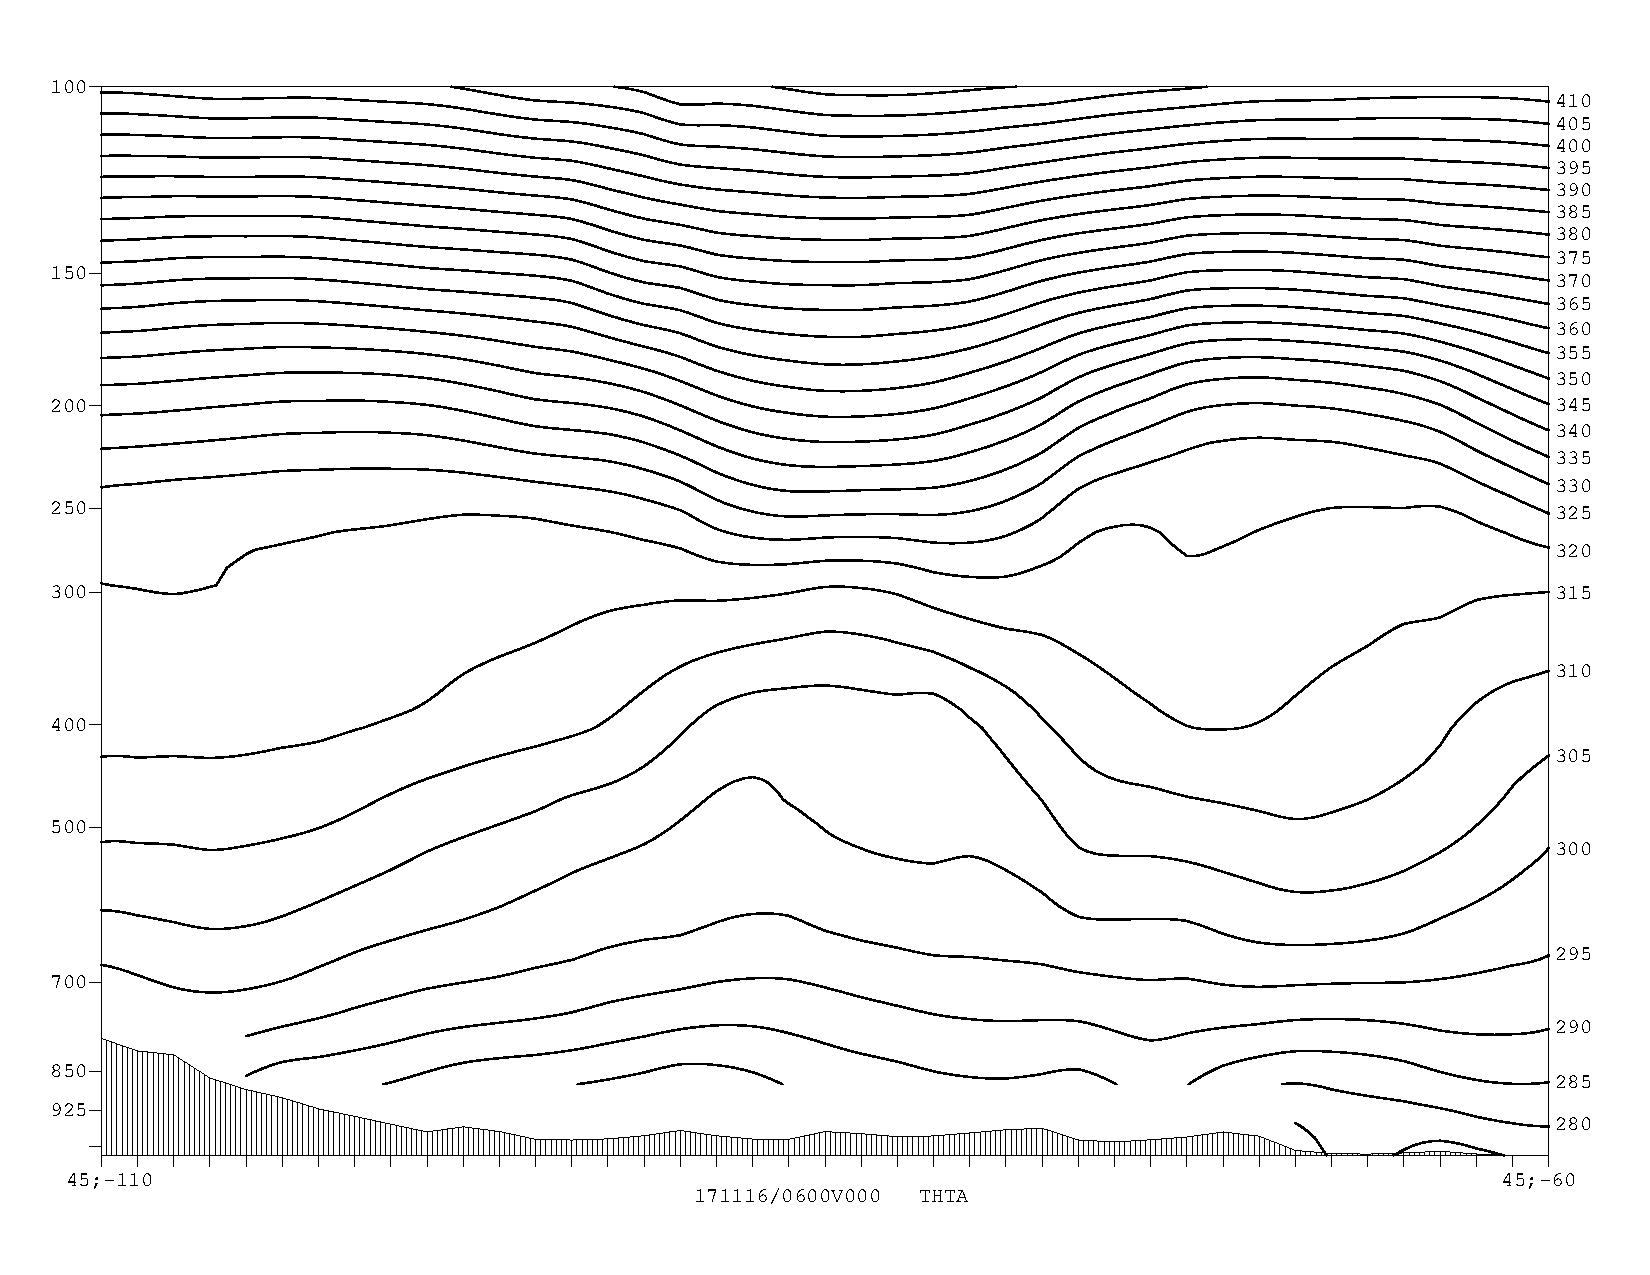
\includegraphics[width=\textwidth]{thta_171116_6Z_moreEast}
  \caption{Zonal cross-section of the potential temperature at \SI{45}{\degree N} and from \SI{110}{\degree W} to \SI{60}{\degree W} on November 16, 2017 6Z (6 hours later).}
  \label{fig:thta_171116_6Z_EW}
\end{figure}


\begin{figure}[h!]
  \centering
  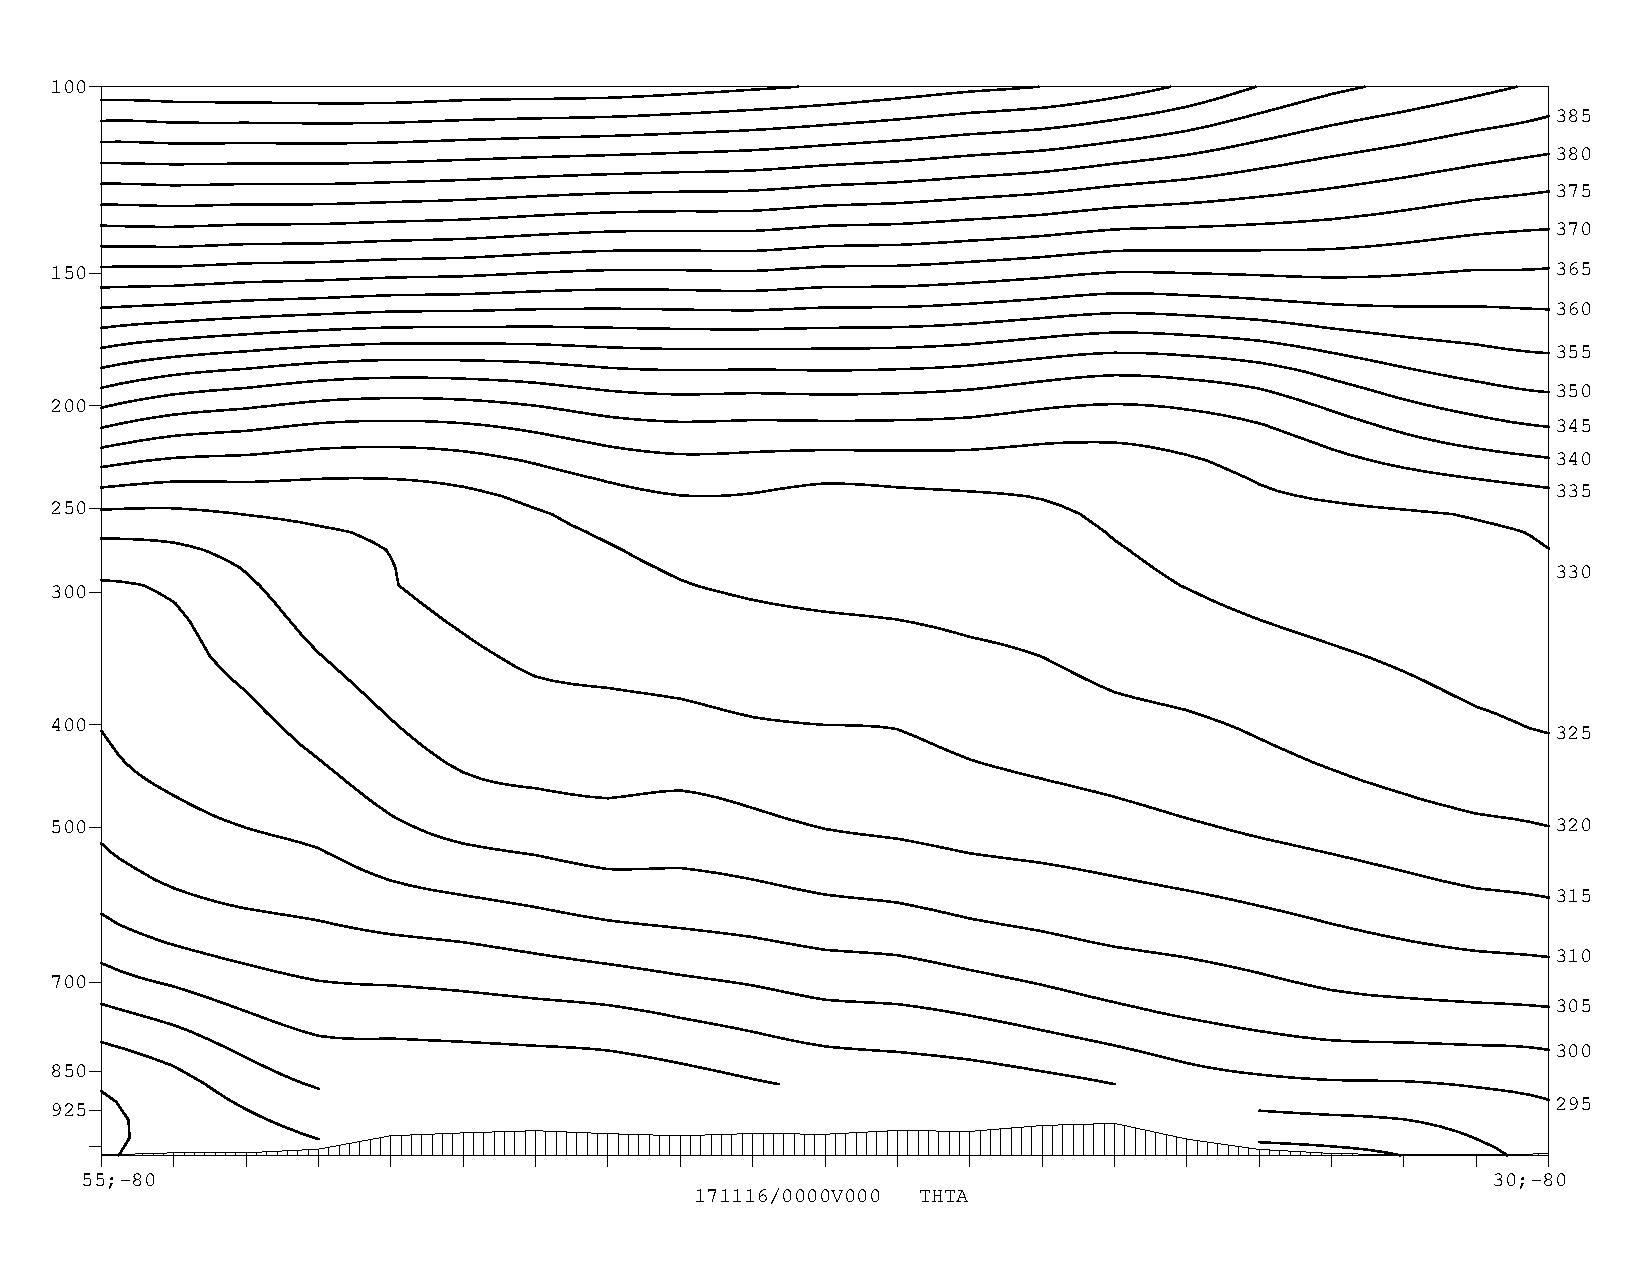
\includegraphics[width=\textwidth]{thta_171116_0Z_NS_lon80W}
  \caption{Meridional cross-section of the potential temperature at \SI{80}{\degree W} and from \SI{30}{\degree N} to \SI{55}{\degree N} on November 16, 2017 0Z.}
  \label{fig:thta_171116_0Z_NS_lon80W}
\end{figure}

\begin{figure}[h!]
  \centering
  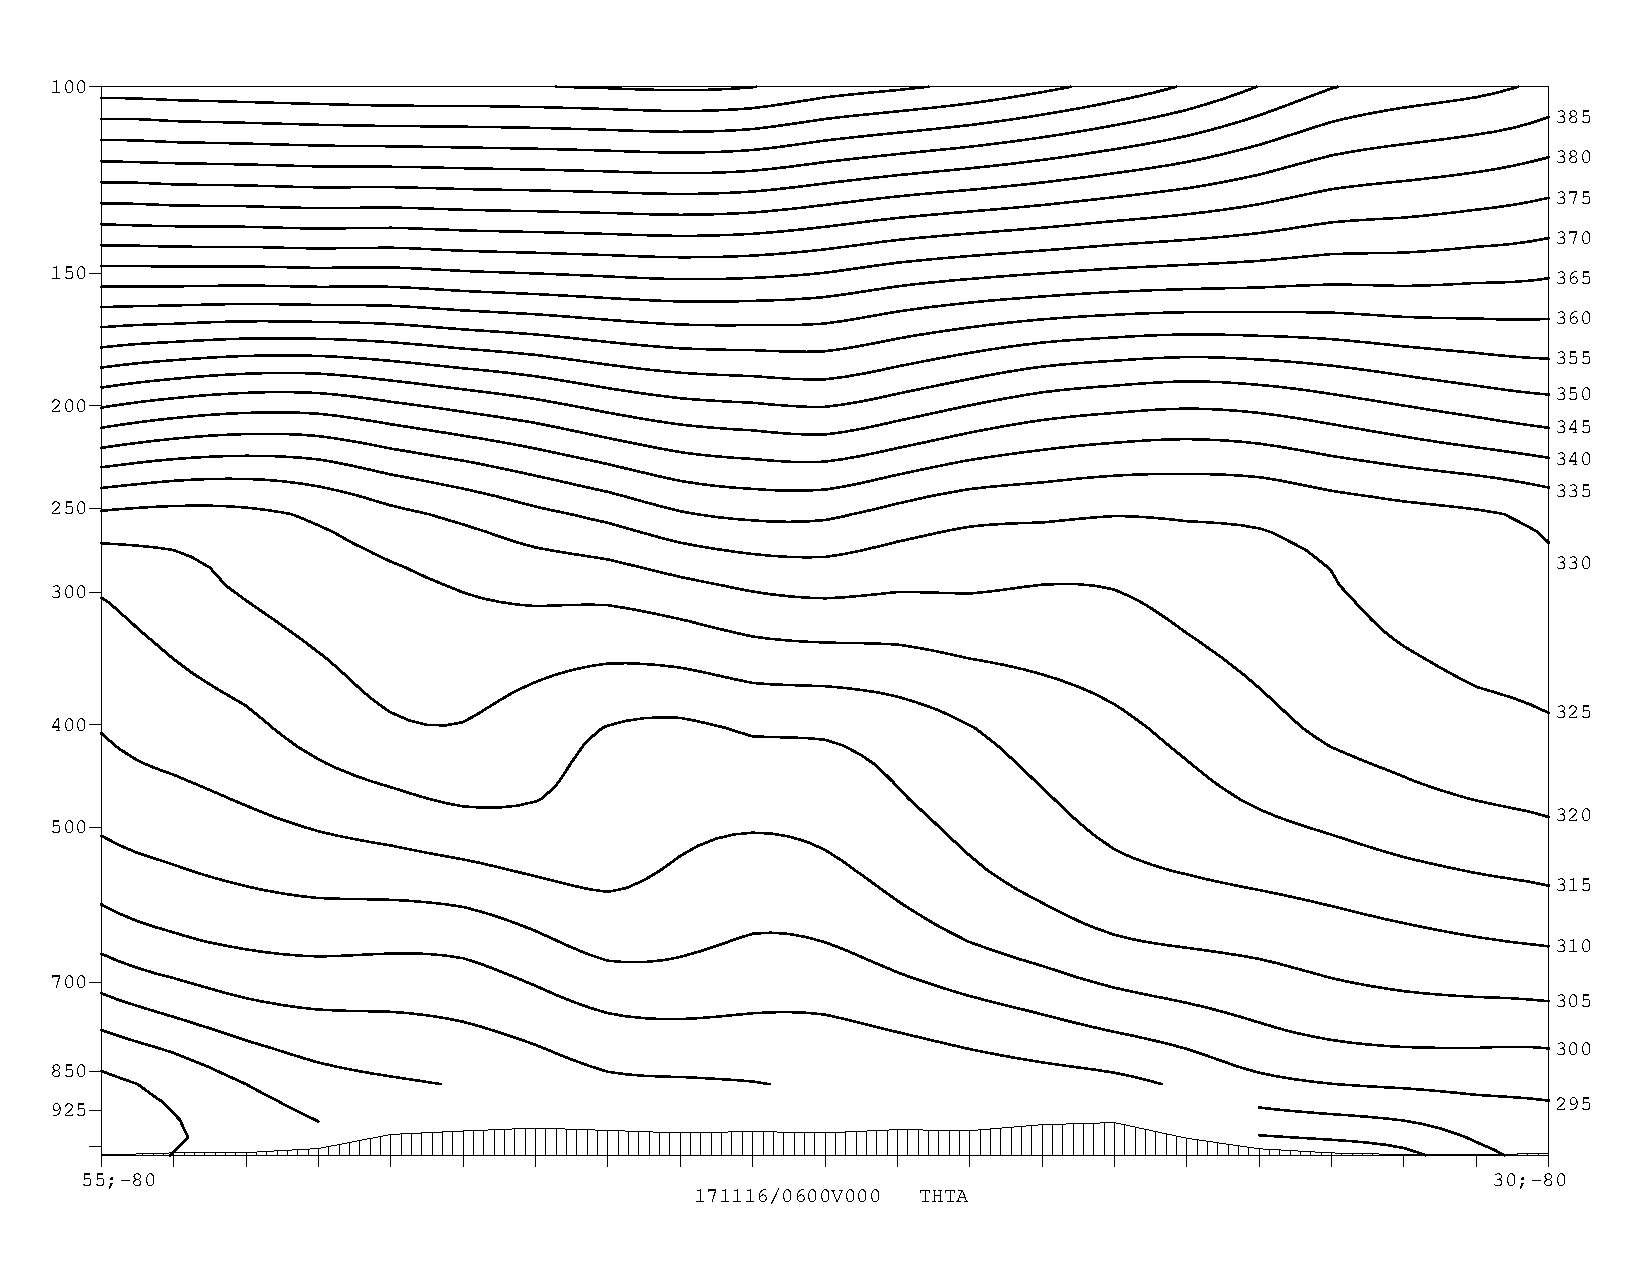
\includegraphics[width=\textwidth]{thta_171116_6Z_NS}
  \caption{Meridional cross-section of the potential temperature at \SI{80}{\degree W} and from \SI{30}{\degree N} to \SI{55}{\degree N} on November 16, 2017 6Z.}
  \label{fig:thta_171116_6Z_NS}
\end{figure}

\begin{figure}[h!]
  \centering
  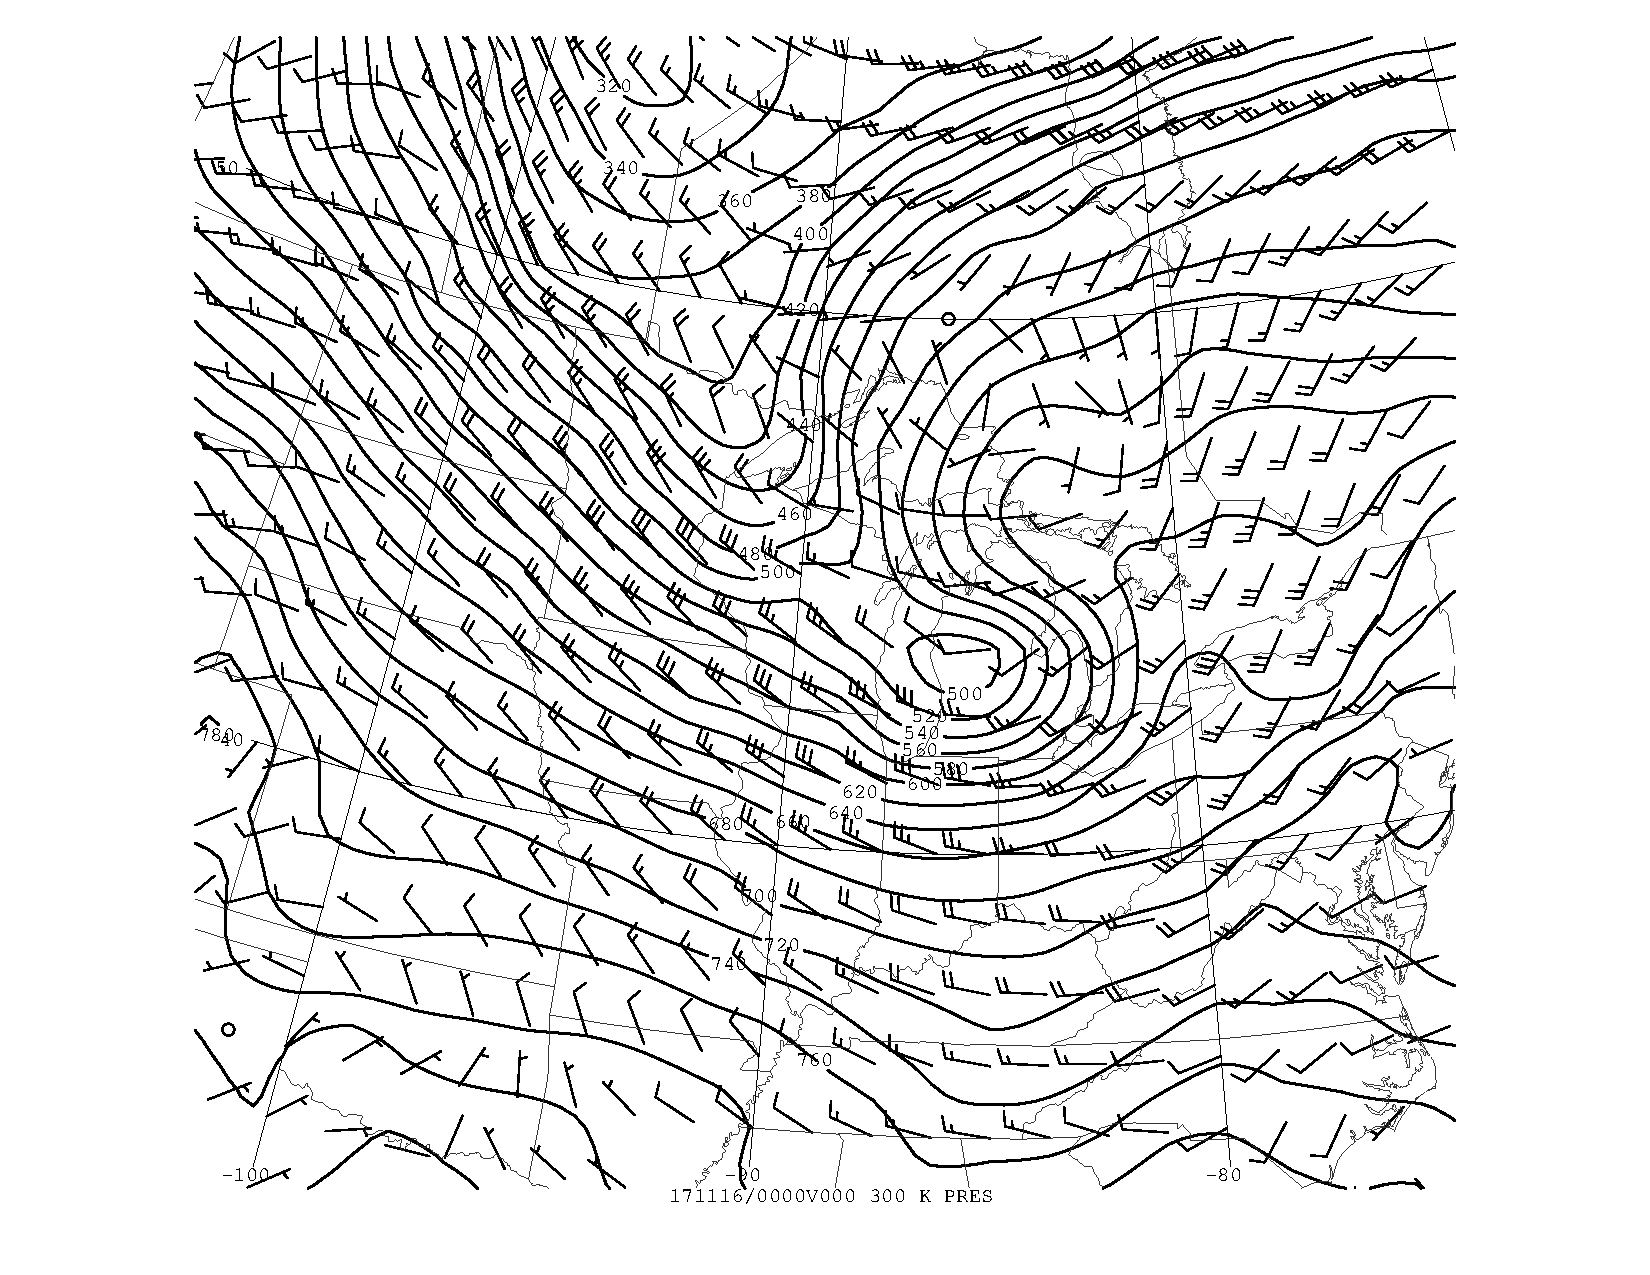
\includegraphics[width=\textwidth,trim={2.5cm 1cm 2.5cm 0},clip]{thta_pres_field_MI_0Z}
  \caption{Contour plot of the pressure at the \SI{300}{\K} potential temperature isentropic surface with the observed wind velocity field superimposed, on November 16, 2017 0Z.}
  \label{fig:thta_pres_field_MI_0Z}
\end{figure}

\begin{figure}[h!]
  \centering
  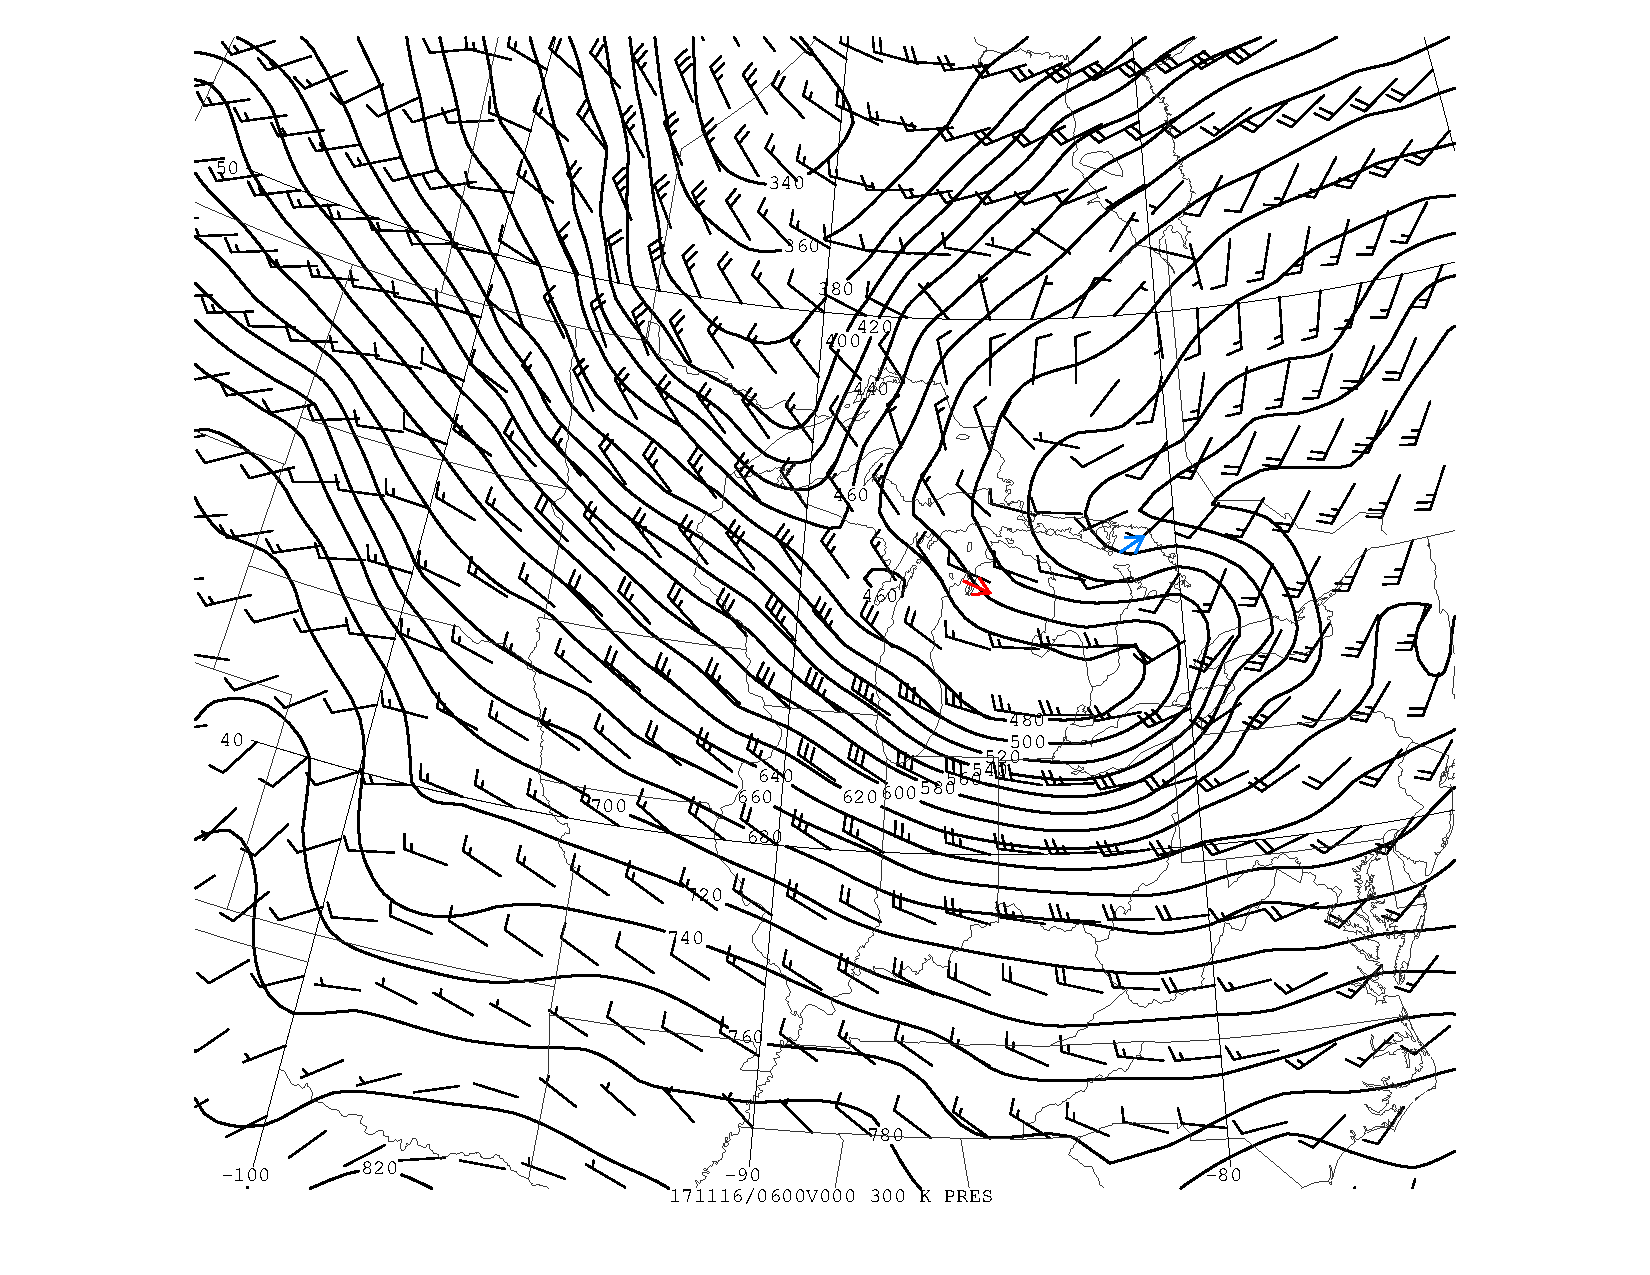
\includegraphics[width=\textwidth,trim={2.5cm 1cm 2.5cm 0},clip]{thta_pres_field_MI_6Z}
  \caption{Contour plot of the pressure at the \SI{300}{\K} potential temperature isentropic surface with the observed wind velocity field superimposed, on November 16, 2017 6Z (6 hours later).}
  \label{fig:thta_pres_field_MI_6Z}
\end{figure}

We use the same locations as the previous section to estimate vertical velocities (see the red and blue circles in figure \ref{fig:omega_MI_850hPa}). We draw the trajectories from 0Z to 6Z using straight blue arrows for the location corresponding to the blue circle and using straight red arrows for the location corresponding to the red circle. The wind velocity is on the order of \SI{10}{\m\per\s} and so the air parcels do not move more than 200--250 km over the six hour period, which is barely one gridpoint across. For the first three hours we evolve the trajectory according to the 0Z field and the second three hours we use the 6Z field.

The red trajectory goes from \SI{530}{\hecto\Pa} at 0Z to \SI{500}{\hecto\Pa} at 6Z corresponding to a vertical velocity of $\omega = -30/6 = \SI{-5}{\Pa\per\s}$, which is pretty close to $\omega = \SI{-4}{\Pa\per\s}$, the observed value and value we calculated using the vorticity equation.

The red trajectory goes from \SI{625}{\hecto\Pa} at 0Z to \SI{570}{\hecto\Pa} at 6Z corresponding to a vertical velocity of $\omega = -55/6 = \SI{-9.2}{\Pa\per\s}$, which is somewhere in between the previously calculated value of \SI{-10.2}{\Pa\per\s} and the observed value of \SI{-7}{\Pa\per\s}. 

One obvious process that might compromise our results are clouds, so it might be more accurate on a clear day.

\end{document}